\RequirePackage[hyphens]{url}
\documentclass{VUMIFPSkursinis}
\usepackage{algorithmicx}
\usepackage{algorithm}
\usepackage{algpseudocode}
\usepackage{amsfonts}
\usepackage{amsmath}
\usepackage{bm}
\usepackage{caption}
\usepackage{color}
\usepackage{float}
\usepackage{graphicx}
\usepackage{listings}
\usepackage{subfig}
\usepackage{wrapfig}
\usepackage{parcolumns}
\usepackage{enumitem}
\usepackage{array}
%PAKEISTA, tarpai tarp sąrašo elementų
\setitemize{noitemsep,topsep=0pt,parsep=0pt,partopsep=0pt}
\setenumerate{noitemsep,topsep=0pt,parsep=0pt,partopsep=0pt}
\renewcommand{\lstlistingname}{Kodo ištrauka}

% Titulinio aprašas
\university{Vilniaus universitetas}
\faculty{Matematikos ir informatikos fakultetas}
\department{Programų sistemų katedra}
\papertype{Kursinis darbas}
\title{WebAssembly panaudojamumo galimybių analizė kuriant internetines programas }
\titleineng{WebAssembly Usability Analysis in Web Development}
\status{3 kurso 5 grupės studentas}
\author{Kasparas Taminskas}
\supervisor{Lekt. Aurimas Šimkus}
\date{Vilnius – \the\year}

% Nustatymai
%\setmainfont{Palemonas}   % Pakeisti teksto šriftą į Palemonas (turi būti įdiegtas sistemoje)
\bibliography{bibliografija}

\begin{document}
\lstset{language=C}

% PAKEISTA	
\maketitle
\cleardoublepage\pagenumbering{arabic}

%TURINYS
\setcounter{page}{2}
\tableofcontents

\sectionnonum{Įvadas}
Interneto naudojimo reikšmė ir taikymo sritys per 30 paskutiniųjų metų nuo žiniatinklio atsiradimo išaugo 
eksponentiškai – šiomis dienomis programinės įrangos kūrimo rinkoje internetinės technologijos ir 
platformos, debesų kompiuterija yra įmonių dėmesio centre, nes galimybė pasiūlyti programinį 
produktą internetu atveria didelį konkurencinį pranašumą – klientams nebereikia įsidiegti 
programinės įrangos į savo elektroninius įrenginius, užtenka vienos programos – interneto 
naršyklės – atveriančios plačias galimybes naudotis skirtingų tipų programomis, pateikiamomis 
kaip paslauga klientui (angl. — Software as a Service). Be to, patys programų sistemų kūrėjai 
patiria mažesnius kaštus kurdami ir palaikydami savo produktus, nes nebelieka poreikio turėti 
skirtingų kodo bazių specifinėms operacinėms aplinkoms ar įrenginiams.

Poreikis turėti kompleksiškas programų sistemas internetinėje erdvėje kelia didelius 
reikalavimus pagrindiniams saityno technologijų kūrėjams – didiesiems naršyklių gamintojams – 
kurių technologinės naujovės įgalina programuotojus įgyvendinti programinius sprendimus 
internete: šios naujos kartos programos internete turi užtikrinti tokius pačius kokybinius 
reikalavimus — greitaveiką, saugumą ir patikimumą — kaip senosios. Šioje vietoje susiduriama 
su dideliais technologiniais naršyklių variklių implementacijos ir pagrindinės internetinių 
technologijų programavimo kalbos – JavaScript – ribojimais, neleidžiančiais įgyvendinti 
internetinių programų visiško supanašėjimo su tradicinėmis, veikiančiomis specifinėse 
platformose. 

Šiame rašto darbe nagrinėjamas naujas WebAssembly atvirų standartų rinkinys, kurio siūlomos naujovės turėtų leisti ženkliai sumažinti likusius techninius barjerus tarp 
naujos kartos internetinių programų sistemų ir tradicinių, nuo vykdymo aplinkos priklausomų 
sprendimų ir atverti saityne dar neišnaudotas rinkos perspektyvas, sėkmingai gyvuojančias
tradicinėse platformose. 

\textbf{Darbo tikslas} – identifikuoti skirtingus scenarijus, kaip standartas 
gali būti integruotas į naujas ir jau egzistuojančias internetines programų sistemas. Kiekvienam scenarijui siekiama pagrįsti jo taikymo racionalumą ir palyginti jo esminius skirtumus su tradiciniu, iki šiol taikytu kūrimo požiūriu.

Išsikelti pagrindiniai tarpiniai uždaviniai, padedantys atskleisti WebAssembly standarto esmę ir įgyvendinti užsibrėžtą tikslą:
\begin{itemize}
    \item \textbf{Identifikuoti kintančią saityno naudojimo paskirtį}
    \item \textbf{Apibrėžti interneto naršyklių programinio kodo vykdymo principus}
    \item \textbf{Išskirti WebAssembly technologijos veikimo logikos ypatybes} 
    \item \textbf{Išbandyti WebAssembly kodo generavimo ir vykdymo procesą, susipažinti su šiomis dienomis egzistuojančiais iššūkiais}
    \item \textbf{Surasti ir aprašyti keletą skirtingų WebAssembly pritaikymo galimybių}
\end{itemize}

\section{Žiniatinklio naudojimo paskirties raida}

Siekiant geriau suprasti dabartinę padėtį, kurioje buvo pristatytas WebAssembly standartas ir kokius poreikius jis patenkina, yra būtina apžvelgti viso žiniatinklio populiarumo augimą ir jo technologinę raidą, lėmusią pakitusią interneto naudojimo paskirtį.

\subsection{Interneto populiarumo augimas}

Interneto bendruomenę sudarančių Žemės gyventojų skaičius šiuo metu viršija pusę visos Žemės populiacijos. Šis augimas, prasidėjęs 1995 metais, kai Saitynas atsivėrė plačiai pasaulio bendruomenei, nesustoja ir toliau, tą galima pastebėti iš \ref{fig:internet_usage} paveikslėlyje matomos viešos metinės statistikos.

\begin{figure}[h!]
  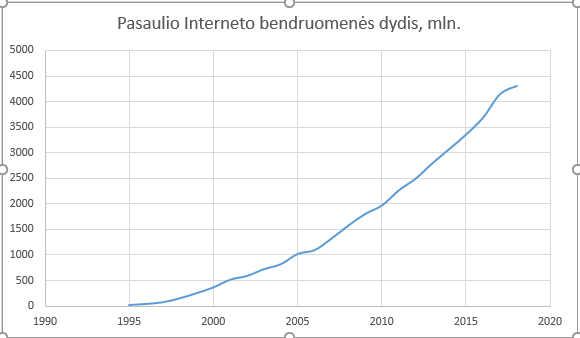
\includegraphics[scale=1]{interneto_naudojimo_statistika.png}
  \caption{Interneto bendruomenės narių skaičius 1995—2018 \cite{IWS19}}
  \label{fig:internet_usage}
\end{figure}

Ši statistika tik patvirtina plataus Interneto technologijų pritaikymo poreikio aktualumą ir didelę atsakomybę, tenkančią šių technologijų kūrėjams — interneto naršyklių gamintojams. Žiniatinklis jau seniai nėra skirtas tik informacijos paieškai ir dalinimuisi, ką įgalino pradinės saityno technologijos — OSI\footnote{angl. Open Systems Interconnection - koncepcinis protokolų kategorizacijos modelis} modelio aplikacijos lygio HTTP\footnote{angl. Hyper Text Transfer Protocol} protokolas, HTML\footnote{angl. Hyper Text Markup Language} ir CSS\footnote{angl. Cascading Style Sheets} žymėjimo kalbos. Ši žiniatinklio paskirties kitimo raida aiškiai atsispindi iš semantinės saityno kategorizacijos, kurią pasiūlė Pasaulinio žiniatinklio konsorciumo pirmininkas, saityno įkūrėjas Tim-Berners Lee.

\subsection{Semantinės Saityno stadijos}
Šiuo metu pagal viešai priimtą, žiniatinklio įkūrėjo Sero Tim-Berners Lee apibrėžtą kategorizaciją, yra išskirtos trys pagrindinės semantinės Saityno stadijos, nurodančios palaipsniui augančią žiniatinklio technologijų poreikio svarbą \cite{NS09}.

\subsubsection{Saitynas 1.0}
Ši semantinė kategorija apibrėžia ankstyvąjį žiniatinklį, kuris geriausiai nusakomas kaip kontekstinėmis nuorodomis sujungtų dokumentų visuma, pasiekiama naudojant interneto naršyklę. Šis apibrėžimas nurodo, jog Saitynas yra itin statiškas, skirtas tik pasiekti ir skaityti informaciją, kurią publikuoja proporcingai sąlyginai maža interneto bendruomenės narių dalis.

\subsubsection{Saitynas 2.0}
Ši kategorija apibrėžiama kaip revoliucinis etapas, kai Saitynas suteikia galimybes ne tik pasiekti, bet vis plačiau dalintis ir kurti informaciją internetinėje erdvėje kiekvienam jos bendruomenės nariui. Pagrindinis skirtumas nuo pirmosios semantinės versijos, jog informacijos sklaidos kryptis tapo dvipusė. Žemiau lentelėje pateikiama keletas esminių Saityno technologijų, lėmusių platesnį informacijos kūrimą ir dalinimąsį ja, priskiriamų šiai semantinei versijai: 

\begin{table}[H]
  \centering
  \caption{Saityno 2.0 technologijos}
  {\begin{tabular}{|m{13em}|m{13em}|} \hline
     Technologija & Paaiškinimas \\
    \hline
    Socialiniai tinklai & Pavyzdžiai - Facebook, Twitter, Instagram platformos. Informacija dalinasi ir kuria kiekvienas tinklo bendruomenės narys.\\
 \hline
Elektroninė komercija &
     Virtualios parduotuvės, elektroninės valdžios vartai, konsultavimas internetu. Šio tipo technologijos kuria Interneto ekonominę erdvę ir generuoja milžiniškas pajamas kiekvienais metais\\
    \hline
     Programinės paslaugos & Programiniai resursai internete, leidžiantys naudotis kompiuterine programine įranga debesų kompiuterijos pagrindu. Pavyzdžiui - Gmail pašto paslauga, Dropbox bylų saugojimo ir dalinimosi įrankis \\
     \hline
  \end{tabular}}
  \label{tab:kompiliavimas_interpretavimas}
\end{table}

\subsubsection{Saitynas 3.0}
Šis etapas apibrėžia kintantį požiūrį į informaciją, pasiekiamą žiniatinklyje. Internetas tampa viena didele duomenų baze, skirta ne tik pavieniams individams ar organizacijoms valdyti duomenis, tačiau daugiau jais dalintis tarpusavyje, interpretuoti ir perteikti įvairiomis perspektyvomis. Tradicinis interneto svetainės konceptas pamažu netenka prasmės, nes visa viešai žiniatinklyje prieinama informacija gali būti pasiekiama ir toms programų sistemoms, kurios tiesiogiai nefunkcionuoja internetinėje erdvėje.

\subsection{Besiplečiančio žiniatinklio iššūkiai}
Identifikuotas kompleksiškų programų sistemų poreikio augimas interneto erdvėje kelia aukštus reikalavimus jau egzistuojančioms pagrindinėms žiniatinklio technologijoms - interneto naršyklėms, jų viduje esantiems JavaScript kalbos varikliams, apdorojantiems ir vykdantiems programinį išeities kodą. Dažnu atveju su turimomis technologijomis šie reikalavimai tampa per sudėtingi ir neįgyvendinami. Norint suprasti šiuos esamus architektūrinius žiniatinklio technologijų barjerus, reikia suvokti, kaip veikia interneto naršyklės ir kokiu būdu jos vykdo programinio kodo instrukcijas.

\section{Interneto naršyklių programinio kodo vykdymo principai}
Interneto naršyklė architektūriniu požiūriu yra itin sudėtinga programa, nes procese nuo resurso parsiuntimo iš nutolusio serverio iki jo grafinio atvaizdavimo naršyklės lange dalyvauja daug sisteminių programos komponentų, nurodytų \ref{fig:browser_architecture} paveikslėlyje. 

\begin{figure}[h!]
  \begin{center}
  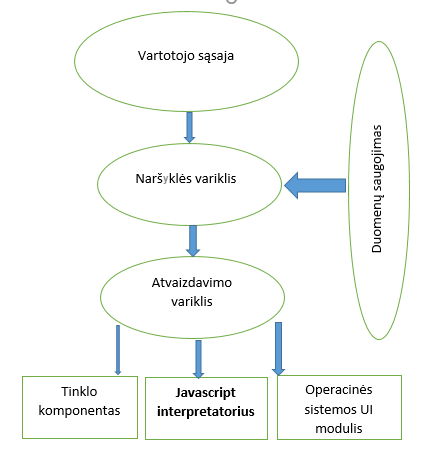
\includegraphics[scale=0.8]{naršyklės_architektūra.png}
  \end{center}
  \caption{Aukšto lygio interneto naršyklės veikimo principas \cite{Rag17}}
  \label{fig:browser_architecture}
\end{figure}

Vienas esminių šios schemos komponentų — JavaScript interpretatorius — žiniatinkliui suteikia dinamiškumą ir leidžia vykdyti skriptus, parašytus JavaScript programavimo kalba, tiesiog naršyklėje. Interpretatoriaus rezultatai siunčiami atvaizdavimo varikliui, kuris pasirūpina jų išdėstymu interneto programoje. \cite{Rag17} Norint geriau suprasti JavaScript vykdymo greitaveikos problemas, būtina suvokti interpretavimo trūkumus, todėl apžvelgsime du fundamentaliai skirtingus programinio kodo transliavimo į mašininį kodą principus.

\subsection{Transliavimo metodai}
Programinės kalbos dažniausiai skirstomos į statines ir dinamines, t.y. ar programiniai tipai egzistuoja kompiliavimo metu, ar yra nustatomi kodo vykdymo metu. Keletas šioms skirtingoms šeimoms priklausančių kalbų:
\begin{enumerate}
    \item Statinės: C, C++
    \item Dinaminės: Python, Rust, JavaScript
    \item Turinčios abejų šeimų požymių: Java, C\#
\end{enumerate} Pagal tai, kuriai šeimai kalba priklauso, skiriasi būdas, kuriuo išeities kodas yra verčiamas į mašinines tam tikros architektūros procesoriaus instrukcijas.

\subsubsection{Kompiliavimas ir interpretavimas}
\ref{tab:kompiliavimas_interpretavimas} lentelėje pateikti šių transliavimo metodų skirtumai ir ypatumai, atskleidžiantys konkretaus metodo privalumus ir trūkumus tam tikrose situacijose. Būtina pažymėti, kad universalaus sprendimo, kuris variantas geresnis, nėra, todėl programavimo pasaulyje derinami abu variantai.

\begin{table}[H]
  \centering
  \caption{kompiliavimo ir interpretavimo skirtumai \cite{PRO19}}
  {\begin{tabular}{|m{13em}|m{13em}|} \hline
     Kompiliavimo savybės & Interpretavimo savybės \\
    \hline
    Transliuojamas visas išeities kodas iš karto & Kodas transliuojamas dalimis 
 sakinys po sakinio \\
 \hline
 Pradinė kodo analizė 
     užima proporcingai didesnę laiko dalį, nei interpretavimo atveju, 
     tačiau vykdymas ženkliai greitesnis &
     Pradinis kodo analizės etapas daug greitesnis, 
     tačiau vykdymo greitaveika lėtesnė   \\
    \hline
     Generuojamas tarpinis objektinis kodas, kuris
 reikalauja surišimo žingsnio, papildomai naudojama atmintis & Nėra generuojama jokio tarpinio kodo \\
 \hline
 Klaidos pranešimas 
 generuojamas tik atlikus pilną kodo analizę, derinimo žingsnis daug sunkesnis &
 Programa transliuojama iki pirmos klaidos, kuomet 
 vykdymas stabdomas, todėl programos derinimas lengvas  \\
 \hline
  \end{tabular}}
  \label{tab:kompiliavimas_interpretavimas}
\end{table}

\subsection{JavaScript kalbos savybės}

Nuo pat žiniatinklio atsiradimo pradžios interneto technologijų branduolį sudaro JavaScript programavimo kalba, kurios prototipas per 10 dienų buvo sukurtas 1995 metais kompanijos Netscape Communications \cite{Ast15}. Ši programavimo kalba žiniatinklyje iki šiol užėmė visišką monopoliją, interneto aplikacijų klientinės dalies kūrimas be jos yra tiesiog sunkiai įsivaizduojamas atvejis. Kalbos populiarumą ir išplitimą patvirtina GitHub saugyklos repozitorijų statistiniai duomenys, pagal kuriuos kalba jau ilgą laiką pirmauja turėdama virš 320000 aktyvių repozitorijų. \cite{GIT19}

\subsubsection{Dinaminė prigimtis}

JavaScript programavimo kalba pasižymi dinaminiais tipais, t.y. kintamieji savo reikšmių tipus gali keisti skripto vykdymo metu. Žemiau pateikta kodo ištrauka yra visiškai validi ir leidžiama interpretatoriaus:

\begin{center}
\begin{small}
\begin{verbatim}
var x = 10;                   //console.log(x) => 10
x = "sveiki";                 //console.log(x) => sveiki
x = {                         //console.log(x) => [Object]
    a: "sveiki iš objekto",
    b: 10,
    c: true
}
\end{verbatim}
\end{small}
\end{center}

Ši kalbos savybė programuotojams užtikrina lanksčias galimybes greitai ir ekspresyviai rašyti programinį kodą, kurio vykdymo pradžia yra itin greita, nes JavaScript yra interpretuojama kalba. Deja, bet ši kalbos dinamiškumo savybė itin trukdo vykdyti programinį kodą, kuris imlus operacijų kiekiui, reikalauja didelės greitaveikos, nes interpretatorius privalo kiekvieną kartą tikrinti, ar vykdomas kodas turi tuos pačius tipus, monitoringo procesas yra imlus greitaveikai. \cite{Cla17}

\subsection{Naršyklių gamintojų greitaveikos problemos sprendimas}


Didieji naršyklių gamintojai siekdami išnaudoti geriausias interpretatorių ir kompiliatorių savybes įdiegė naujus papildomus žingsnius JavaScript kodo vykdymo variklyje. Dauguma JavaScript variklių šiuo metu naudoja labai panašios architektūros kodo kompiliavimo procesus, todėl panagrinėsime vieno jų — Google kompanijos kuriamo ir palaikomo atviro kodo variklio — veikimo principus.

\subsubsection{V8 variklio JavaScript kodo vykdymo etapai}
\begin{figure}[h!]
  \begin{center}
  \includegraphics[scale=0.8]{V8_kompiliavimo_grandinė.png}
  \end{center}
  \caption{V8 JavaScript variklio kodo vykdymo grandinė \cite{Kad19}}
  \label{fig:v8_pipeline}
\end{figure}

Iki 2008 metų JavaScript kodo vykdymas naršyklėse buvo pastebimai lėtesnis, tačiau prasidėjus naršyklių gamintojų „greitaveikos karams" buvo įdiegti JIT (angl. — Just in Time) kompiliatoriai, kurie pastebimai padidino greitaveikos rodiklius. \cite{Cal17} Šių kompiliatorių vietą JavaScript kodo vykdymo grandinėje galima matyti \ref{fig:v8_pipeline} paveikslėlyje.
JIT kompiliatoriai kodą optimizuoja pagal sukauptą informaciją iš monitoringo įrankio, kuris stebi kintamųjų tipus, jų kitimą, funkcijų kvietimo dažnius ir kt. Jeigu optimizuotas kodas tampa nevalidus (tarkime, jog atėjo nauji kintamųjų tipai), atliekamas deoptimizavimo žingsnis, JavaScript kodo vykdymas grąžinamas V8 interpretatoriui - Ignition. Šis procesas reikalauja laiko, todėl, žinoma, kenčia ir kodo vykdymo greitaveika, tačiau gana stabiliam kodui optimizavimo procesas naudingas.
\subsubsection{Ribojimai}
Nepaisant šių technologinių naujovių naršyklių varikliuose, optimizavimo procesas vykdant JavaScript kodą dažnai neatitinka keliamų poreikių. Tas puikiai matosi pritaikant vaizdo apdorojimo algoritmus, skirtus tam tikram efektui išgauti. Pavyzdžiui, kadrų skaičius per sekundę, JavaScript kalba realizavus Super Edge Inv\footnote{Vaizdo efekto algoritmas, išryškinantis objekto kontūrus} vaizdo efekto algoritmą, yra pastebimai žemas ir juntamas aiškus uždelsimas. \cite{WVE17} Reikalinga naujovė, kuri leistų internete išgauti tokią pačią greitaveiką, kuri sėkmingai taikoma programuojant su tradicinėmis platformomis, pavydžiui, OpenGL\footnote{Programinė sąsaja, skirta manipuliuoti vektorine 2D ir 3D grafika} grafine biblioteka ir statine kompiliuojama C++ kalba.

\section{WebAssembly standarto specifikacija}

WebAssembly yra standartų rinkinys, sukurtas ir palaikomas Pasaulio žiniatinklio konsorciumo (angl. — World Wide Web Consorcium), apibrėžiantis koncepcinį žemo lygio mašinio kodo formatą, į kurį gali būti verčiamos aukšto lygio programavimo kalbos. \cite{WAS17}

\subsection{Programavimo kalbos ypatybės}
WebAssembly yra žemo lygio, statinė programavimo kalba, turinti vos keletą kintamųjų tipų:

\begin{itemize}
    \item Sveikojo skaičiaus: i32, i64
    \item Slankaus kablelio: f32, f64
\end{itemize}
Lyginant šią kalbą su JavaScript, kuri yra dinaminė, aukšto lygio, galima pastebėti, jog nėra tokios įvairovės ir lankstumo — jokių eilučių tipų, masyvų, objektų. Funkcijų parametrų ir grįžimo reikšmės privalo būti griežtai deklaruotos ir apibrėžtos. Taip pat WebAssembly specifikacijoje apibrėžti statiniai užvardinti funkcijų importavimai ir eksportavimai.


\subsection{Koncepcinio mašininio kodo vykdymas}
WebAssembly mašininis kodas skirtas vykdyti steko pagrindu veikiančioms virtualioms mašinoms. Virtuali mašina yra aukšto lygio abstrakcijos sluoksnis, leidžiantis programinį kodą vykdyti skirtingose operacinėse sistemose ir fizinėse architektūrose, todėl WebAssembly mašininį kodą lyginti su tradiciniu konkrečios fizinės architektūros mašininiu kodu būtų neteisinga. \cite{Cal17} Supaprastinta WebAssembly programinio kodo vertimo į konkrečią fizinę architekūrą schema pateikta \ref{fig:wasm_compilation} paveikslėlyje. Programinės kalbos dažnai turi tarpines kodo išraiškas (angl. — Intermediate Representation), skirtas programinį kodą versti į konkrečios fizinės architektūros mašinininį kodą. WebAssembly mašininis kodas sugeba priimti šį tarpinį formatą, naršyklių implementacijos sugeba atlikti WebAssemly kodo transliavimą į konkrečią fizinę architektūrą be sudėtingų ir laikui imlių žingsnių. 

\begin{figure}[h!]
  \begin{center}
  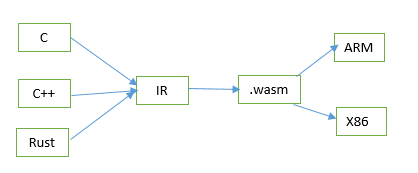
\includegraphics[scale=1]{webassembly_kompiliavimas.png}
  \end{center}
  \caption{WebAssembly kodo kompiliavimas \cite{Cla17}}
  \label{fig:wasm_compilation}
\end{figure}

\subsection{Virtualios mašinos realizacija}

WebAssembly formatas sukurtas steko pagrindu veikiančiai mašinai — tai specialus virtualios mašinos implementacijos atvejis, kai aritmetiniai ir loginiai operandai ir operacijų rezultatai saugomi steko pagrindo duomenų struktūroje, o išėmimo ir įdėjimo tvarka grįsta LIFO\footnote{angl. Last In First Out - paskutinis idėtas bus pirmas išimtas} principu. 

\begin{figure}[h!]
  \begin{center}
  \includegraphics[scale=1]{sudėtis_steke.png}
  \end{center}
  \caption{Sudėtis steke}
  \label{fig:stack_addition}
\end{figure}

Šis virtualios mašinos implementacijos būdas užtikrina efektyvią greitaveiką, nes nereikia išreikštinai žinoti operandų atminties adresų — naudojama steko viršūnės rodyklė (angl. — Stack Pointer), o kiekiena įdėjimo/išėjimo operacija pakeičia šios rodyklės reikšmę vienetu.
Kaip matome \ref{fig:stack_addition} paveikslėlyje, paprastai sudėties operacijai steko implementacijos atveju reikia keturių komandų. Egzistuoja registrais grįsta virtualios mašinos realizacija, kurioje sudėtis gali būti išreiškiama viena operacija, tačiau tokiu atveju reikia nurodyti ir žinoti registrų adresus, todėl užimama daugiau vietos. \cite{Sin12} Neteisinga teigti, jog viena implementacija universaliu atveju geresnė už kitą, efektyvumą lemia naudojimo kontekstas.

\subsection{Atviras standartų rinkinys}
WebAssembly technologija yra standartizuota, todėl nereikalauja papildomų įskiepių ar kitų programinių papildinių. Visos modernios naršyklės — Chrome, Safari, Edge, Firefox — realizavusios WebAssembly vykdymo variklius, todėl programuotojams nebereikia spręsti skirtingų naršyklių suderinamumo problemos, kuri dažnai itin išaugina programavimo laiko ir kainos kaštus. Tiesa, reikia paminėti, jog šis standartas nepalaikomas Internet Explorer naršyklėse. 

Šiame skyriuje aptartos WebAssembly standarto greitaveiką lemiančios kalbos žemo lygmens, statiškumo ir greižtos išraiškos savybės, vidinė virtualios mašinos steko pagrindu realizacija, todėl toliau galima ieškoti konkrečių technologijos pritaikymo erdvių.

\section{WebAssembly panaudojamumo būdai}
Standarto panaudojimo galimybes kuriant interneto programas galima skirstyti pagal pritaikymo skalę — kokią proporcinę visos programos kiekio dalį užima WebAssembly kodo bazė.

\subsection{Modulio integracija į egzistuojantį JavaScript projektą}
Dar iki WebAssembly standarto atsiradimo, nuo ECMAScript2015 standarto specifikacijos išleidimo, JavaScript ekosistema tapo daug moduliaresnė, nei buvo prieš tai \cite{Cla17}. Ši technologinė savybė leidžia enkapsuliuoti realizacijos logiką, o klientui pateikti tik ribotą programinę sąsają (angl. — Application Programming Interface), skirtą naudotis paketu ar moduliu. WebAssembly standartas kuriamas atsižvelgiant į modulių naudą ir poreikį.

\subsubsection{Problemos apibrėžimas}
Sakykime, jog turime realizavę internetinę programą, kurios esminė verslo logikos dalis atlieka procesoriaus ar vaizdo plokštės darbo laikui imlias operacijas. Mūsų klientai džiaugiasi, jog esame pirmieji realizavę tokio tipo sistemą internete, tačiau skundžiasi, jog darbas su sistema nėra sklandus, juntamas dažnas uždelsimas. Tokių sistemų pavyzdžiai galėtų būti vaizdo, garso kodavimo ir apdorojimo programos, papildytos realybės (angl. — Augmented Reality) sprendimai, dirbtinio intelekto sistemos. 
\subsubsection{Sprendimas}
Galima bandyti susidariusią problemą spręsti pertvarkant egzistuojantį centrinį verslo logikos algoritmą, parašytą JavaScript programavimo kalba ir stebint greitaveikos rodiklius, tačiau anksčiau ar vėliau neabejotinai bus pasiekta riba, kurios peržengti su esama technologija nebus įmanoma, nes pati kalba nesuteikia prieigos prie žemų programinių konstruktų, tokių kaip savarankiškas ir efektyvus atminties išskyrimas ir valdymas. 
\subsubsubsection{WebAssembly integracija}
Šioje vietoje atsiranda galimybė panaudoti enkapsuliuotą WebAssembly modulį, kuris savyje turėtų realizuotą centrinį skaičiavimų logikos algoritmą \cite{Cal17}. Jeigu mūsų internetinės programų sistemos sprendimas kilo iš jau anksčiau egzistavusios darbalaukinės programos, didelė galimybė, jog mums net nereikės perrašinėti jokios verslo logikos kita kalba, galėsime sukompiliuoti seną kodo bazę į \verb|.wasm| mašininio kodo formatą ir iškviesti programinį modulį tiesiai iš interneto naršyklės. Šis seno kodo pernaudojimo principas suteikia galimybę išnaudoti WebAssembly technologinės naujovės teikiamą naudą net nemokant programuoti tomis kalbomis, kurių bibliotekas ar modulius norime panaudoti. Sakykime, jog savo algoritmą turime įgyvendinę C programavimo kalba, imituokime mūsų verslo logikos funkcionalumą realizuodami paprastą Burbulo metodo (angl. — Bubble Sort) rikiavimo funkciją:

\begin{center}
\begin{small}
\begin{verbatim}
int8_t* EMSCRIPTEN_KEEPALIVE bubbleSort(int8_t *buf, int n) {
    for (int i=0; i<n—1;i++) {
        for (int j=0;j<n—i—1;j++) {
            if (buf[j]>buf[j+1]) {
                swap(&buf[j], &buf[j+1]);
            }
        }
    }
    return buf;
}
\end{verbatim}
\end{small}
\end{center}

Verta paminėti, jog \verb|EMSCRIPTEN_KEEPALIVE| direktyva nurodo, jog šią funkciją reikia įtraukti į WebAssembly eksportuojamų funkcijų sąrašą, tuomet ją bus galima kviesti tiesiai iš JavaScript programinio kodo. \cite{EMD17}

Kai jau turime parašę savo centrinį verslo logikos algoritmą, esminis žingsnis — šį išeities kodą paversti binariniu \verb|.wasm| formato moduliu, kurį galėtume importuoti naršyklėse. Patogiausias ir plačiausiai taikomas rinkoje įrankis — Emscripten atviro kodo kompiliatorius. Savo darbalaukinėje sistemoje sudiegę šį įrankį, komandinėje eilutėje galime iškviesti kompiliavimo komandą:

\begin{center}
\begin{small}
\begin{verbatim}
emcc bubble_sort.c —s WASM=1 —s EXPORTED_FUNCTIONS="['_bubbleSort']" 
—s "EXTRA_EXPORTED_RUNTIME_METHODS=['ccall','cwrap']"
\end{verbatim}
\end{small}
\end{center}
Kompiliavimo komandos sintaksė skiriasi priklausomai nuo naudojamos operacinės sistemos, šiuo atveju buvo naudojama Windows 10 operacinė sistema ir jos komandinė eilutė.

Įvykdžius terminalo lango komandą įrankis sugeneruoja \verb|.wasm| modulį ir \verb|.js| failą, kuris skirtas inicijuoti WebAssembly modulio vykdymą naršyklėje. Naršyklių gamintojai teigia, jog planuose yra patogesnis \verb|.wasm| modulio integravimas taikant tradicinį modulių importavimo požiūrį: \verb|<script type="module"></script>|. Deja, tačiau rašymo metu ši galimybė dar neegzistuoja, todėl modulio užkrovimas naršyklėje reikalauja gana didelio kiekio surišančiojo JavaScript kodo, kurį sugeneruoja minėtasis Emscripten įrankis.

Šiame pavyzdyje C funkcijai iš JavaScript kodo turime perduoti masyvą ir jo elementų ilgį, kad galėtume per jį iteruoti. Kol kas tiesioginis parametrų perdavimas galimas tik su primityviaisiais skaitiniais tipais, jeigu norime perduoti masyvą, turime pasitelkti piramidės struktūrą (angl. — Heap Data Strcuture). 
\begin{figure}[h!]
  \begin{center}
  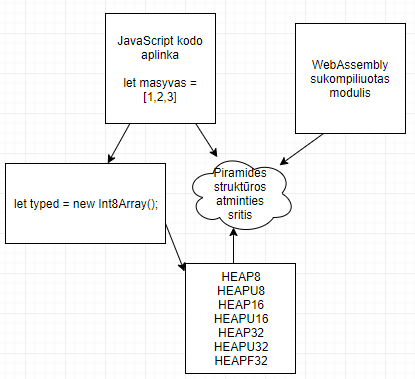
\includegraphics[scale=1]{wasm_heap.png}
  \end{center}
  \caption{WebAssembly ir JavaScript komunikacija naudojant piramidės atmintį}
  \label{fig:wasm_stack}
\end{figure}
Ši atminties sritis WebAssembly standarte yra tiesiog paprastas JavaScript objektas, kuris imituoja tradicinę C/C++ kalbų piramidės duomenų struktūrą, nes pastarosios pasiekti dėl saugumo priežasčių programuotojai galimybės neturi. 
Sudėtingų tipų perdavimą tarp JavaScript kodo ir WebAssembly modulio galima pavaizduoti \ref{fig:wasm_stack} paveikslėlyje nurodyta schema, kurioje matosi, jog komunikacija tarp aplinkų vyksta netiesiogiai, žiūrint į bendrą atminties sritį.

Svarbu paminėti, jog negalime į piramidę tiesiogiai patalpinti apibrėžto JavaScript masyvo, turime jį paversti į tipizuotą masyvo tipą, atitinkantį konkretaus tipo piramidę, nes vieno tipo piramidėje negalima laikyti skirtingo tipo duomenų — kitu atveju bus gaunami netikėti ir nesąmoningi rezultatai. 

Taigi, turėdami sukompiliuotą modulį ir jį iškviečiantį sugeneruotą surišantįjį JavaScript kodą, galime bandyti iškviesti aprašytą C rikiavimo funkciją iš naršyklės. Šiam tikslui naudojame integruotas WebAssembly standarto realizacijos \verb|Module.ccall()| ir \verb|Module.cwrap()| funkcijas, leidžiančias perduoti parametrus į WebAssembly modulį ir grąžinti rezultatą į JavaScript aplinką atgal. Šiame pavyzdyje naudojame \verb|wasm—arrays.js| atviro kodo biblioteką, patalpintą GitHub saugykloje, kuri suteikia papildomą \verb|ccall| ir \verb|cwrap| funkcijų abstrakcijos lygmenį, skirtą patogesniam naudojimui. \cite{WAA19} Taigi, naršyklės kode galime iškviesti mūsų rikiavimo funkciją perduodami skaičių masyvą:

\begin{center}
\begin{small}
\begin{verbatim}
        const res = ccallArrays(
          "bubbleSort",
          "array",
          ["array"],
          [[2, 1, 13, 4, 50]],
          { heapIn: "HEAP8", heapOut: "HEAP8", returnArraySize: 5 }
        );
        console.log(res);
\end{verbatim}
\end{small}
\end{center}

Pirmuoju parametru nurodome kviečiamą funkciją, antrasis parametras apibrėžia iš kviečiamos funkcijos grįžtantijį tipą, trečias ir ketvirtas — perduodamų parametrų tipus ir reikšmes, penktasis parametras — perduodamas objektas — apibrėžia jog naudosime WebAssembly \verb|HEAP8| (baito dydžio) sveikųjų skaičių piramidės atminties sritį. Įvykdžius \verb|ccallArrays| funkciją rezultato kintamasis \verb|res| gauna \verb|int8_t| tipo rodyklę, būtent tokio tipo, kokį apibrėžėme C funkcijoje. Ši rodyklė rodo į surikiuoto masyvo pradžios atminties sritį, todėl JavaScript kode galime pasiekti pakeistąjį masyvą. Našyklės konsolėje stebimas \ref{fig:sorted_array} paveikslėjyje matomas funkcijos kvietimo rezultatas.

\begin{figure}[h!]
  \begin{center}
  
\includegraphics[scale=1]{sorted_array.png}
  \end{center}
  \caption{Rezultatas naršyklės konsolės lange}
  \label{fig:sorted_array}
\end{figure}

Tagi, šiame pavyzdyje sugebėjome realizuoti logikos algoritmą C programavimo kalba, jį sukompiliuoti į WebAssembly modulį ir iškviesti JavaScript kode. Ši situacija parodo, jog WebAssembly standarto moduliarumo savybė leidžia skaičiavimams jautrias logikos sritis perkelti iš JavaScript kodo į WebAssembly modulius. Būtent todėl WebAssembly standartas ne pakeičia, o papildo JavaScript veikimą ten, kur pokytis atrodo racionalus ir reikalingas.

\subsubsection{Realaus pasaulio scenarijai}

Aprašytasis pavyzdys tik vaizdžiai parodo, kaip galima WebAssembly integruoti į egzistuojančią interneto sistemą pagerinant greitaveikos rodiklius. Interneto programų sistemų rinkoje jau galime pastebėti esančius tokio moduliarumo taikymo pavyzdžius.

Galimas pavyzdys — architektų plačiai naudojama Autodesk kompanijos kuriama projektavimo programa AutoCAD, kurios kodo bazė C++ kalba pradėta kurti dar 1982 metais. Kompanija nuolat stengėsi vis didesnę savo programos logiką perkelti į internetinę programų sistemą, tam tikslui buvo pasitelkusi dabar jau nebegyvuojančią Adobe kompanijos Flash įskiepių technologiją. WebAssembly moduliai leido kompanijai neperrašinėti egzistuojančios verslo logikos, o tiesiog ją sukompiliuoti į mašininį \verb|.wasm| kodą. Rezultatas — žiniatinklyje egzistuojantis programinis sprendimas, kurio galimybės beveik lygios tradiciniam programiniam paketui \cite{Che18}.

Kitas pavyzdys, kuris rinkoje jau implementuotas — kompanijos eBay programuotojų komandos sukurta internetinė brūkšninio kodo nuskaitymo programa, skirta eBay aukciono pardavėjams įkelti savo parduodamas prekes. Šis įrankis eBay programuotojų buvo sukurtas C++ kalba ir sėkmingai veikė iOS ir Android mobiliose aplinkose. Atsiradus WebAssembly technologijos realizacijai interneto naršyklėse, eBay programuotojai egzistuojančią kodo bazę sukompiliavo į \verb|.wasm| modulį, rezultatas buvo stebinantis — lyginant su anksčiau veikusiu JavaScript brūkšninio kodo nuskaitymo įrankiu, kuris veikdavo vieno kadro per sekundę režimu, WebAssembly realizacija leido pasiekti 50 kartų didesnę greitaveiką. \cite{Hea19}

\subsubsection{Galimi egzistuojančių projektų patobulinimai}
Vienas tokių atvejų galėtų būti ReactJS biblioteka, skirta kurti klientiniam interneto kodui. Esminis šios bibliotekos suderinimo (angl. — Reconciliation) algoritmas, skirtas efektyviai perpiešti DOM medį ir pastebėti, kurie šio medžio lapai pakeitė būseną, galėtų būti pakeistas WebAssembly realizacijos kodu išlaikant tokį patį programinį kontraktą React bibliotekos naudojams (angl. — API) \cite{Cla17}. Tokiu atveju vienintelis pokytis, kurį pajustų naudotojai — išaugusi bibliotekos veikimo sparta, bibliotekos naudotojai neturėtų mokytis jokių naujų standarto konstruktų, todėl pasinaudotų jo teikiamais privalumais dažnu atveju to net nežinodami.

\subsection{WebAssembly pagrindu pagrįsto karkaso naudojimas}
Vienas didžiausių standarto privalumų, kurio įtaką žiniatinkliui galima laikyti revoliucine, yra tai, jog WebAssembly mašininio kodo formatas skirtas būti kompiliuojamu iš skirtingų programavimo kalbų. Tai reiškia, jog JavaScript kalbos monopolis kuriant klientines interneto programas baigėsi. Anksčiau kuriant klientinę žiniatinklio sistemos dalį buvo būtina turėti plačias JavaScript kalbos ir ja parašytų karkasų ir bibliotekų, tokių kaip React, Angular, Vue taikymo žinias. Neteisinga teigti, jog JavaScript žinių nuo šiol nebereiks, tačiau žiniatinklyje vis daugiau vietos atsiras ir kitoms programavimo kalboms, kurias buvo įprasta matyti programuojant serverinę sistemos dalį. Faktas, jog visa klientinė programos logika perkeliama vykdyti į WebAssembly modulius leidžia beveik išsisukti be JavaScript kodo rašymo jį pakeičiant tradiciškai serverio dalies kodo rašymui skirta programavimo kalba:

\begin{center}
\begin{small}
\begin{verbatim}
@page "/skaitliukas"
<p>Dabartinis skaicius: @currentCount</p>
<button onclick="@IncrementCount">Padidinti</button>
@functions {
    int currentCount = 0;
    void IncrementCount()
    {
        currentCount++;
    }
}
\end{verbatim}
\end{small}
\end{center}Pateiktas C\# Razor sintaksės pavyzdys, kuriame paspaudus mygtuką skaitliukas padidinamas vienetu \cite{BLZ19}. Dažniausiai tokį kodą dinamiškai vykdo JavaScript variklis, tačiau, kaip matome iš pavyzdžio, viskas rašoma naudojant tik HTML ir C\#, šiame pavyzdyje nedaroma jokių HTTP užklausų į nutolusį serverį.

Šis WebAssembly pritaikymo pavyzdys yra daug platesnis nei anksčiau aprašytasis centrinės logikos realizacijos pakeitimo, nes apima visą klientinės programos logikos perkėlimą į WebAssembly mašininį kodą.

Naujo karkaso kūrimo galimybes ir iššūkius naudojant WebAssembly kodą galima suprasti įsigilinus į jau realizuotus pavyzdžius, kurie, nors vis dar ankstyvose stadijose, tačiau jau nusako kryptį, kurios bus laikomasi.

\subsubsection{Egzistuojantys WebAssembly pagrindu veikiantys karkasai}
Nors WebAssembly technologija dar tebėra pradiniuose kūrimo etapuose, rinkoje jau pateikta keletas variantų, leidžiančių išbandyti naują patirtį kuriant vieno puslapio internetines aplikacijas (angl. - Single Page Applications) su tradiciškai serverio programiniam kodui rašyti skirtomis kalbomis.
\subsubsubsection{Microsoft .NET Blazor karkasas}
Microsoft kompanijos kuriamas .NET Blazor produktas — vartotojo sąsajos kūrimo C\# programavimo kalba karkasas, leidžiantis .NET programos kodui būti vykdomam tiesiogiai naršyklėje. \cite{BLZ19} Ši savybė leidžia programuotojams pernaudoti serverio dalyje esantį .NET kodą kuriant klientines programas.

C\# kalbos kodo vykdymui reikalinga .NET vykdomoji aplinka, todėl esminis Blazor karkaso funkcinis vienetas yra Microsoft Xamarin komandos kuriama ir palaikoma Mono .NET vykdomoji aplinka, skirta mobiliųjų programėlių ir žaidimų konsolinėms platformoms kūrimui naudojant .NET technologijas. Nuo šiol ši vykdomoji aplinka veikia ir interneto naršyklėse — pastaroji buvo sukompiliuota į WebAssembly modulį. Šis modulis su savimi turi ir nebenaudojamų resursų surinkimo konstruktą (angl. — Garbage Collection), leidžiantį programuotojui nesirūpinti rankiniu atminties valdymu programuojant. Aukšto lygio Blazor veikimo principas nurodytas \ref{fig:blazor_architecture} schemoje, kur matome, jog mono.wasm — tai į WebAssembly mašininio kodo formatą sukompiliuota .NET Mono vykdomoji aplinka.

\begin{figure}[h!]
  \begin{center}
  \includegraphics[scale=1]{blazor_veikimo_architektūra.png}
  \end{center}
  \caption{Blazor karkaso veikimas naršyklėje \cite{BLZ19}}
  \label{fig:blazor_architecture}
\end{figure}

Verta paminėti, jog, kaip ir praeitame skyriuje demonstruotame pavyzdyje, kur buvo naudojamas Emscripten pagalba sugeneruotas JavaScript kodas, reikalingas užkrauti WebAssembly moduliui, turime \verb|mono.js| ir \verb|blazor.js| skriptus, reikalingus vykdomosios \verb|mono.wasm| aplinkos užkrovimui. Šis .NET vykdomomios Mono aplinkos režimas yra interpretuojamasis, nes mūsų kurta programa \verb|Programa.dll| nėra sukompiliuota į WebAssembly mašininį formatą, o interpretuojama pačioje kliento naršyklėje \verb|mono.wasm| modulio. Mono aplinka palaiko ir išankstinį (angl. — Ahead of Time) programos vykdymo būdą, kai mūsų kurta programa sukompiliuoajama į WebAssembly modulį iš anksto. Kaip pirmame skyriuje minėta, nėra fundamentaliai aišku, kuris modelis geresnis, tačiau interpretuojamas modelis daug artimesnis programavimui internete, nes kodo pokyčiai atsispindi naršyklės lange beveik iš karto — sukompiliavus pakeistą programos vietą, o taikant išankstinį modelį kompiliavimo žingsnis užtrunka pastebimai ilgiau, tačiau pats veikimo greitis greitaveikai jautriose vietose būna didesnis.

Kuriant serverio pusės logiką ASP.NET technologine platforma nebuvo itin aktuali surinkimo tekstų (angl. — .NET assemblies) užimama disko vieta serveryje — 2 MB ar 50 MB disko vietos užimantis kodas didelio skirtumo nedarydavo, tačiau naršyklės vykdyme šis aspektas yra kritinis, todėl net pritaikius Mono vykdomosios aplinkos ir programos kešavimo mechanizmą, yra itin svarbu, jog pirmasis puslapio užkrovimas, kurio metu parsiunčiama vykdomoji aplinka ir programinis kodas, būtų greitas. Technologijos kūrėjai pripažįsta, kad Blazor programa nesugebės pasiekti tokio suspaudimo lygio, kokį sugeba išgauti ReactJS biblioteka, tačiau pritaikius kelis optimizavimo metodus pasiekiamas rezultatas, leidžiantis galutiniam vartotojui sklandžiai naudotis klientine programa. Keli iš tų metodų yra:
\begin{itemize}
    \item HTTP užklausų atsakymų suspaudimas
    \item Kompiliavimo metu .NET IL surišiklis (angl. — Intermediate Language linker) statiškai skenuoja visą kodą ir pašalina tas dalis, kurios bus nenaudojamos kodo vykdymo metu
    \item .NET vykdomoji aplinka ir programos surinkimo failai kešuojami naršyklėje, kad nereiktų daryti nereikalingų užklausų į nutolusį serverį
\end{itemize}

\subsubsubsection{asm-dom įrankis C++ klientinei programai}
Šis atviro kodo įrankis — virtualaus DOM medžio biblioteka, skirta kurti klientines vieno puslapio aplikacijas C++ programavimo kalba. Ši biblioteka skatina C++ kodo bazės pernaudojamumą ir suteikia kodo vykdymo greitaveiką, kuri artima tradicinėse aplinkose esantiems greičiams \cite{ASM19}. C++ kodas kompiliuojamas į WebAssembly modulius panaudojant jau anksčiau minėtą Emscripten kompiliavimo įrankį.

Ši biblioteka leidžia rašyti programinį kodą naudojant iš ReactJS bibliotekos gerai pažįstamą JSX\footnote{JavaScript sintaksės praplėtimas XML žymėjimo kalbos galimybėmis} sintaksę:

\begin{center}
\begin{small}
\begin{verbatim}
  VNode* vnode = (
    <div
      onclick={[](emscripten::val e) -> bool {
        emscripten::val::global("console")
        .call<void>("log", emscripten::val("paspausta"));
        return true;
      }}
    > </div>
  );
\end{verbatim}
\end{small}
\end{center}
Iš pavyzdžio matome, jog galime iškviesti C++ kodo funkcijas, jas įdėdami kaip JavaScript įvykius apdorojančius metodus. Šis virtualaus DOM medžio įrankis su tikruoju DOM medžiu bendrauja per JavaScript surišantįjį kodą, nes šio rašto darbo rašymo metu WebAssembly technologija vis dar nepalaiko tiesioginės komunikacijos su DOM medžio porgramine sąsaja.

\begin{nopagebreak}
\sectionnonum{Rezultatai}
Rašto darbe pavyko įgyvendinti šiuos rezultatus, susijusius su tikslu ir išsikeltais darbo uždaviniais:
\begin{enumerate}
  \item Nustatyta saityno evoliucinė raida, rodanti augantį žiniatinklio technologijų taikymo poreikį
  \begin{itemize}
  \item identifikuoti žiniatinklio naudotojų kiekio augimo mastai
  \item pristatytos semantinės Saityno raidos versijos
  \end{itemize}
    \item Pristatytas bendras interneto naršyklių JavaScript kodo vykdymo principas
  \begin{itemize}
  \item apibrėžta JavaScript kalbos specifika
  \item palyginti skirtingi kodo transliavimo metodai - kompiliavimas ir interpretavimas
  \item suformuluota bendra JavaScript variklio veikimo schema
  \end{itemize}
  \item Išskirti esminiai WebAssembly standarto aspektai
  \begin{itemize}
    \item akcentuota statinė, žemo lygmens kalbos specifika
    \item nusakytos WebAssembly mašininio kodo formato ypatybės
    \item identifikuota WebAssembly kodą vykdančios virtualios mašinos architektūrinė sudėtis
    \end{itemize}
  \item Išbandytas C kalba parašytos burbulo metodo rikiavimo funckijos kompiliavimo į WebAssembly modulį procesas ir praktiškai išmokta iškviesti sukompiliuotą kodą iš naršyklės perduodant parametrus iš JavaScript aplinkos  į WebAssembly modulį
  \item Darbe pristatyti du pagrindiniai WebAssembly panaudojimo scenarijai
\begin{itemize}
  \item centrinio greitaveikai imlios verslo logikos modulio pakeitimas WebAssembly modulio realizacija
  \item naujos klientinės programos kūrimas nuo pradžių pasitelkiant naujus karkasus, sukurtus WebAssembly technologijos pagrindu
\end{itemize}
\end{enumerate}

\sectionnonum{Išvados}
Iš pasiektų rezultatų galima teigti, jog Saityno ekosistema įgauna vis didesnę reikšmę, siejamą su interaktyvių programų sistemų naudojimu, todėl netolimoje ateityje turėtų būti matomas vis didesnis sistemų migravimas į debesų kompiuterijos erdvę. Atsižvelgiant į tai tampa aišku, jog pristatyta JavaScript kalbos fundamentinė prigimtis ir interneto naršyklėse vykdomi šios kalbos kodo optimizacijos procesai netenkina keliamų greitaveikos ir kodo vykdymo patikimumo reikalavimų, todėl galima teigti, jog apibrėžtas ir pademonstruotas WebAssembly standartų rinkinys pasirodė pačiu laiku, kaip tam tikras minėtų technologinių barjerų rezultatas, siekiantis perimti greitaveikai imlias JavaScript kodo atsakomybės sritis. Nors technologija išlieka pradiniuose kūrimo etapuose ir rašto darbo rengimo metu ganėtinai sunkiai integruojama, pritaikymo galimybės įrodo, jog netolimoje ateityje keisis ne tik kuriamų internetinių sistemų pobūdis, tačiau taip pat bus juntama ir esama tokių sistemų kūrimo suvokimo kaita.

\end{nopagebreak}
%% PAKEISTAS PAVADINIMAS Į 'Šaltiniai'
\addcontentsline{toc}{section}{Šaltiniai} 
\printbibliography[heading=bibintoc, title=Šaltiniai]  % Šaltinių sąraše nurodoma panaudota
\begin{thebibliography}{99}

\bibitem[Abo17]{Abo17} 
Mohammed Aboullaite. Understanding JIT compiler (just-in-time compiler), 2017. Žiūrėta [2019—06—07]. Prieiga internetu: \url{https://aboullaite.me/understanding-jit-compiler-just-in-time-compiler/}

\bibitem[ASM19]{ASM19} 
asm-dom documentation. Žiūrėta [2019—06—07]. Prieiga internetu: \url{https://mbasso.github.io/asm-dom/docs/inline-example.html}

\bibitem[Ast15]{Ast15} 
Ben Aston. A brief history of JavaScript. Žiūrėta [2019—06—07]. Prieiga internetu: \url{https://medium.com/@benastontweet/lesson-1a-the-history-of-javascript-8c1ce3bffb1}

\bibitem[BLZ19]{BLZ19} 
Blazor documentation. Žiūrėta [2019—06—07]. Prieiga internetu: \url{https://docs.microsoft.com/lt-lt/aspnet/core/blazor/?view=aspnetcore-3.0}

\bibitem[Cal17]{Cal17} 
Dan Callahan. Practical WebAssembly, 2017. Žiūrėta [2019—06—07]. Prieiga internetu: \url{http://2017.jsconfbp.com/speakers/dan-callahan/}

\bibitem[Che18]{Che18} 
Kevin Cheung. AutoCAD \& WebAssembly: Moving a 30 Year Code Base to the Web. Žiūrėta [2019—06—07]. Prieiga internetu: \url{https://www.infoq.com/presentations/autocad-webassembly/}

\bibitem[Cla17]{Cla17} 
Lin Clark. A cartoon intro to WebAssembly, 2017. Žiūrėta [2019—06—07]. Prieiga internetu: \url{https://hacks.mozilla.org/2017/02/a—cartoon—intro—to—webassembly/}

\bibitem[EMD17]{EMD17} 
Emscripten documentation. Building to WebAssembly. Žiūrėta [2019—06—07]. Prieiga internetu: \url{https://emscripten.org/docs/compiling/WebAssembly.html}

\bibitem[GIT19]{GIT19} 
A Small Place to Discover Languages In GitHub. Žiūrėta [2019—06—07]. Prieiga internetu: \url{https://githut.info/}

\bibitem[Hea19]{Hea19} 
Nick Heath. Replacing JavaScript: How eBay made a web app 50x faster by switching programming languages, TechRepublic, 2019. Žiūrėta [2019—06—07]. Prieiga internetu:
\url{https://www.techrepublic.com/article/replacing-javascript-with-webassembly-how-ebay-made-a-web-app-50x-faster-by-switching-programming-languages/}

\bibitem[Kad19]{Kad19} 
Yotam Kadishay. JavaScript V8 Engine Explained, 2019. Žiūrėta [2019—06—07]. Prieiga internetu: \url{https://hackernoon.com/javascript-v8-engine-explained-3f940148d4ef/}

\bibitem[NS09]{NS09} 
Umesha Naik, Dr. D. Shivalingaiah. Comparative Study of Web 1.0, Web 2.0 and Web 3.0  Žiūrėta [2019—06—07]. Prieiga internetu: \url{https://www.researchgate.net/publication/264845599_Comparative_Study_of_Web_10_Web_20_and_Web_30}

\bibitem[PRO19]{PRO19} 
Interpreter Vs Compiler : Difference Between Interpreter and Compiler. Žiūrėta [2019—06—07]. Prieiga internetu: \url{https://www.programiz.com/article/difference-compiler-interpreter}

\bibitem[Rag17]{Rag17} 
Monica Raghuwanshi. How does web browsers work?, 2017. Žiūrėta [2019—06—07]. Prieiga internetu: \url{https://medium.com/@monica1109/how-does-web-browsers-work-c95ad628a509}

\bibitem[Sin12]{Sin12} 
Mark Sinnathamby. Stack based vs Register based Virtual Machine Architecture, and the Dalvik VM, 2012. Žiūrėta [2019—06—07]. Prieiga internetu: \url{https://markfaction.wordpress.com/2012/07/15/stack-based-vs-register-based-virtual-machine-architecture-and-the-dalvik-vm/}

\bibitem[TEC19]{TEC19} 
Software as a Service, Definition. 2019. Žiūrėta [2019—06—07]. Prieiga internetu: \url{https://www.techopedia.com/definition/155/software-as-a-service-saas/}

\bibitem[IWS19]{IWS19} 
Internet Growth Statistics, Žiūrėta[2019—06—07]. Prieiga internetu: \url{https://www.internetworldstats.com/emarketing.htm/}

\bibitem[WAA19]{WAA19} 
DanRuta. wasm-arrays. Žiūrėta [2019—06—07]. Prieiga internetu: \url{https://github.com/DanRuta/wasm-arrays}

\bibitem[WAS17]{WAS17} 
WebAssembly Documentation, High Level Goals 2017. Žiūrėta [2019—06—07]. Prieiga internetu: \url{https://webassembly.org/docs/high-level-goals/}

\bibitem[WVE17]{WVE17} 
WebAssembly Video Editor, 2017. Žiūrėta [2019—06—07]. Prieiga internetu: \url{https://d2jta7o2zej4pf.cloudfront.net/}

\bibitem[W3C19]{W3C19} 
Pasaulinio žiniatinklio konsorciumo svetainė. Žiūrėta [2019—06—07]. Prieiga internetu: \url{https://www.w3.org/wiki/Main_Page}

\end{thebibliography}

\sectionnonum{Sąvokų apibrėžimai}

\textbf{Programa kaip paslauga (angl. Software as a Service)} - programinis produktas, nereikalaujantis, jog vartotojas jį įdiegtų į savo elektroninį įrenginį, dažniausiai veikiantis paskirstytuose dalykiniuose serveriuose, duomenų centruose, galintis vienu metu aptarnauti daug vartotojų \cite{TEC19}.

\textbf{Naršyklės smėliadėžės aplinka (angl. browser sandbox environment)} - naršyklėse įdiegta, izoliuota JavaScript ir WebAssembly kodo vykdymo erdvė, ribojanti prieigą prie sisteminių resursų siekiant apsaugoti galutinį interneto naršyklės naudotoją.

\textbf{Pasaulinio žiniatinklio konsorciumas (W3C)} - tarptautinis programinės įrangos kūrimo bendruomenės susivienijimas, kuriantis ir teikiantis standartus ir rekomendacijas žiniatinkliui. \cite{W3C19}

\textbf{Išankstinis kompiliavimas (angl. Ahead-Of-Time Compilation)} - kodo transliavimo į mašinines instrukcijas metodas, paplitęs tarp statinių programavimo kalbų, pasižymintis tuo, jog kodas išverčiamas į mašinines instrukcijas iš anksto, prieš vykdant programinį kodą. \cite{Abo17}

\textbf{Kompiliavimas vykdymo metu (angl. Just-In-Time Compilation)} - dinaminis kodo transliavimo į mašinines instrukcijas metodas, kombinuojantis interpretavimo ir išankstinio kompiliavimo savybes. Vyksta kodo vykdymo metu, vertinama, ar kompiliuojamo kodo vykdymo nauda bus didesnė už kompiliavimo proceso laiko ir atminties kaštus \cite{Abo17}.
\end{document}
